% !TeX program = xelatex
\documentclass[10pt,aspectratio=169]{beamer}
\usepackage{fontspec}
\setmainfont{Cambria}[
  Path=fonts/,
  UprightFont=cambria.ttc,
  BoldFont=cambriab.ttf,
  ItalicFont=cambriai.ttf,
  BoldItalicFont=cambriaz.ttf
]
\usepackage{poly}
\usepackage{booktabs}
\usepackage{colortbl}
\usepackage[spanish]{babel}

% Colores para tablas (usados en celdas destacadas)
\definecolor{verdemejor}{rgb}{0.56, 0.93, 0.56}
\definecolor{rojomenor}{rgb}{1.0, 0.71, 0.76}

% ================================================================================
% Metadata
% ================================================================================

\title{Evaluación comparativa de clasificadores de machine learning para la detección de cáncer de mama}
\author{Carlos Mora, Juan Felipe Rodríguez, Sergio Duarte}
\institute[UDFJC]{Universidad Distrital Francisco José de Caldas -- Analítica de Datos}
\date{Mayo 2026}

% ================================================================================
% Main Body
% ================================================================================

\begin{document}
\maketitle

% ------------------------------------------------------------------------------
\section{Introducción}
% ------------------------------------------------------------------------------

\begin{frame}{Contexto}
\begin{columns}
\begin{column}{0.6\textwidth}
\begin{block}{El problema}
\begin{itemize}
  \item Cáncer de mama: el más frecuente a nivel mundial.
  \item Principal causa de muerte oncológica en mujeres.
  \item \textbf{Supervivencia >90\%} si se detecta en estadios tempranos.
\end{itemize}
\end{block}

\vspace{0.5em}
\begin{block}{La oportunidad}
\begin{itemize}
  \item ML clasifica muestras celulares con resultados comparables o superiores a especialistas.
  \item La clasificación bayesiana permite cuantificar probabilidades de diagnóstico.
\end{itemize}
\end{block}
\end{column}

\begin{column}{0.4\textwidth}
\begin{figure}
\centering
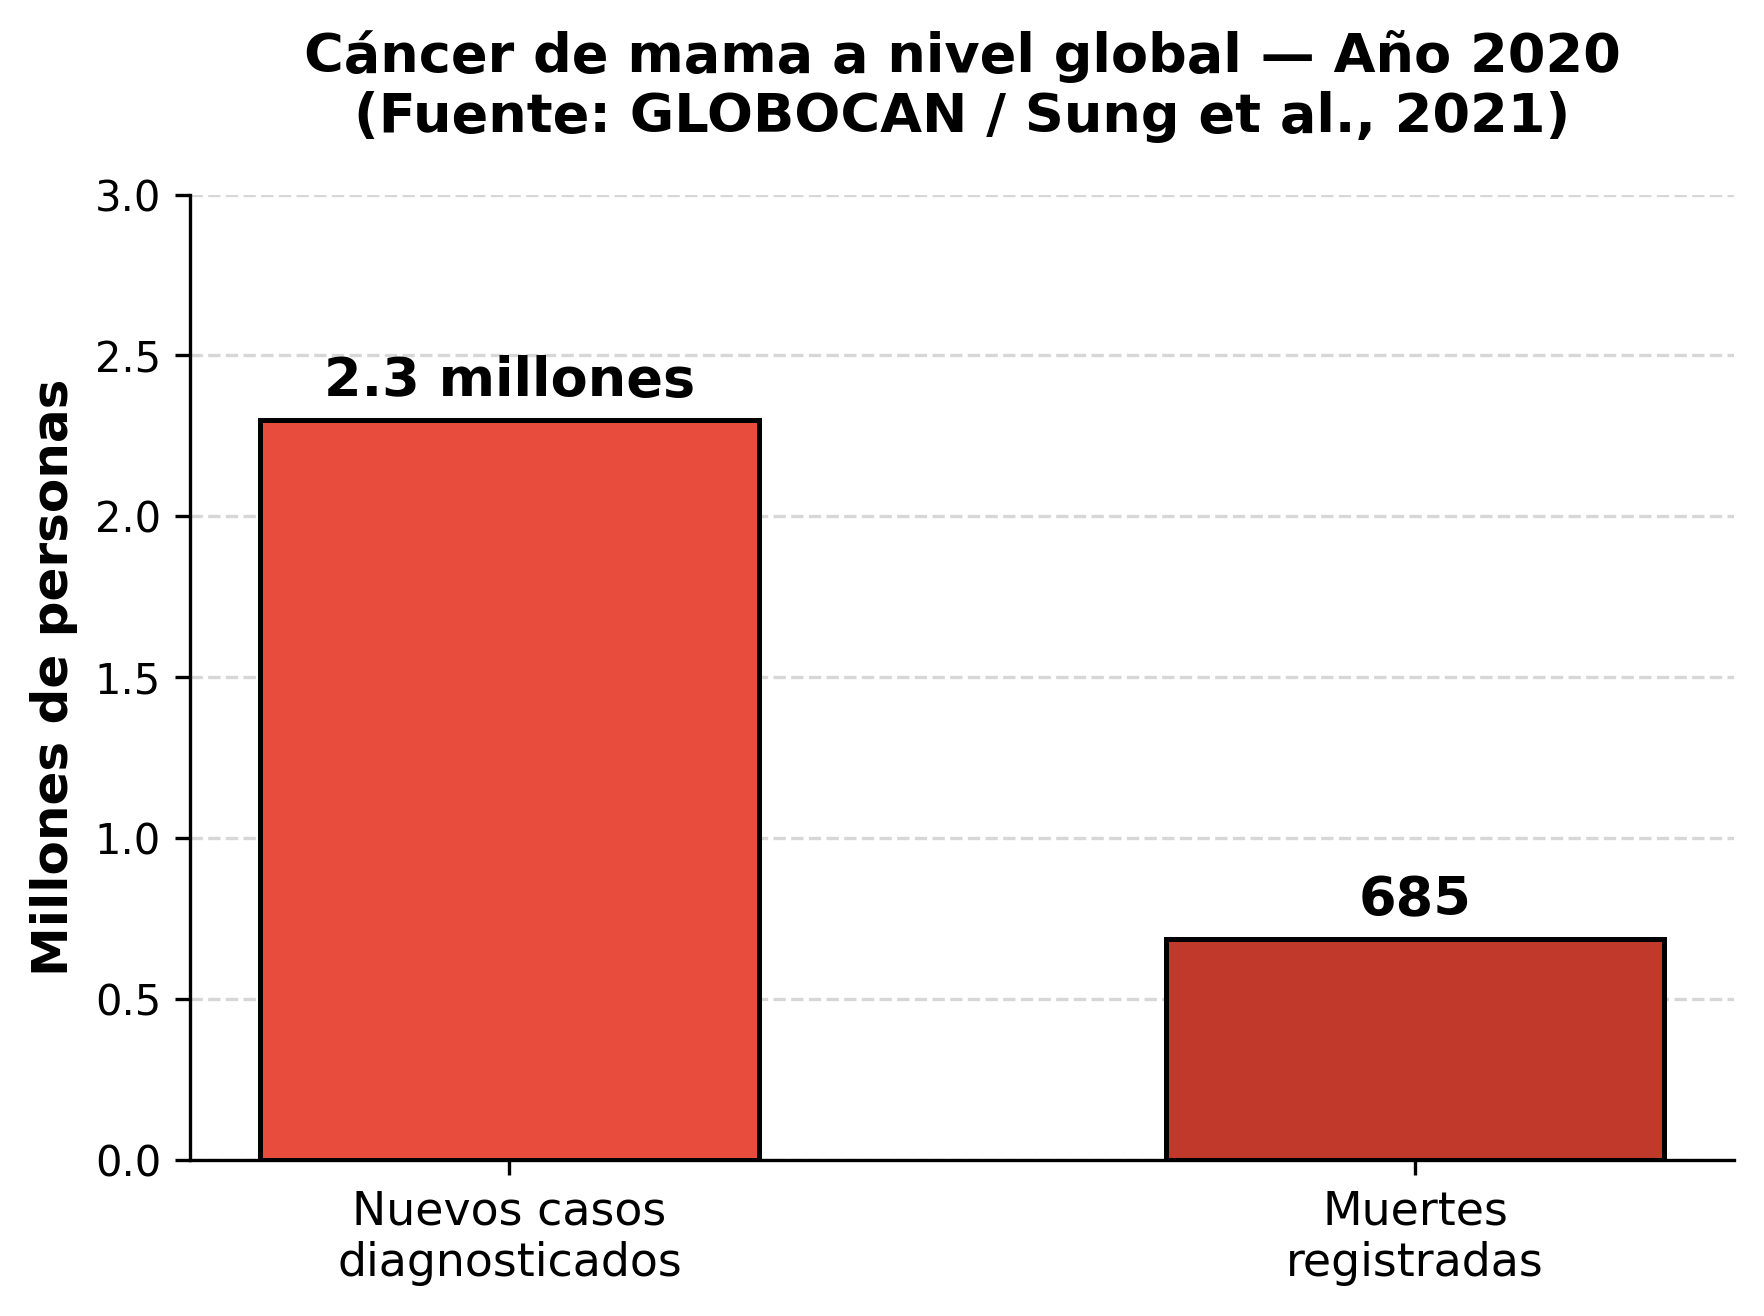
\includegraphics[width=0.9\textwidth]{../documento/images/fig_global_stats_2020.png}
\end{figure}
\end{column}
\end{columns}
\end{frame}

\begin{frame}{Motivación}
\begin{alertblock}{El diagnóstico actual tiene grietas}
La efectividad de los modelos depende del flujo completo:
\begin{itemize}
  \item \textbf{Selección de atributos} -- ¿qué variables realmente importan?
  \item \textbf{Normalización} -- ¿las escalas afectan el modelo?
  \item \textbf{Métricas adecuadas} -- ¿accuracy basta en medicina?
\end{itemize}
\end{alertblock}

\vspace{1em}
\textbf{Este trabajo:} un flujo integrado de analítica de datos evaluando \textbf{9 clasificadores} con métricas clínicamente relevantes.
\end{frame}

% ------------------------------------------------------------------------------
\section{Problemática}
% ------------------------------------------------------------------------------

\begin{frame}{¿Por qué esto importa?}
\begin{columns}
\begin{column}{0.5\textwidth}
\begin{block}{Cifras 2020 (GLOBOCAN)}
\begin{itemize}
  \item 2.3 millones de nuevos casos
  \item 685,000 muertes
  \item Colombia: 140,000+ casos prevalentes
  \item 4,322 defunciones en 2023
\end{itemize}
\end{block}
\end{column}

\begin{column}{0.5\textwidth}
\begin{block}{El diagnóstico por FNA}
Depende de la \textbf{evaluación subjetiva} del patólogo.

\vspace{0.5em}
\textbf{Tasa de discordancia inter-observador:} 15--20\% en casos limítrofes.
\end{block}
\end{column}
\end{columns}

\vspace{1em}
\begin{columns}
\begin{column}{0.5\textwidth}
\begin{exampleblock}{Falso Negativo}
Tumor maligno como benigno $\rightarrow$ \textbf{no tratar} a quien lo necesita.
\end{exampleblock}
\end{column}

\begin{column}{0.5\textwidth}
\begin{block}{Falso Positivo}
Tumor benigno como maligno $\rightarrow$ exámenes innecesarios y ansiedad.
\end{block}
\end{column}
\end{columns}
\end{frame}

% ------------------------------------------------------------------------------
\section{Objetivos}
% ------------------------------------------------------------------------------

\begin{frame}{Objetivos del proyecto}
\begin{block}{Objetivo General}
Implementar un flujo de analítica de datos para la clasificación de tumores mamarios, evaluando nueve clasificadores de Machine Learning sobre el dataset WDBC con el \textbf{Recall de la clase Maligno} como métrica principal.
\end{block}

\vspace{1em}
\begin{block}{Objetivos Específicos}
\begin{enumerate}
  \item Preprocesamiento riguroso: detección de anómalos, normalización, selección de atributos.
  \item Comparar 9 clasificadores bajo condiciones experimentales idénticas.
  \item Analizar estabilidad mediante validación cruzada 5-fold.
\end{enumerate}
\end{block}
\end{frame}

% ------------------------------------------------------------------------------
\section{Dataset}
% ------------------------------------------------------------------------------

\begin{frame}{Wisconsin Breast Cancer Diagnostic Dataset}
\begin{columns}
\begin{column}{0.55\textwidth}
\begin{block}{Características}
\begin{itemize}
  \item \textbf{569 instancias}: 357 benignas (62.7\%) y 212 malignas (37.3\%)
  \item \textbf{30 características numéricas continuas}
  \item Calculadas a partir de imágenes FNA
  \item Variable objetivo: Maligno (1) / Benigno (0)
  \item \textbf{Sin valores faltantes}
\end{itemize}
\end{block}
\end{column}

\begin{column}{0.45\textwidth}
\begin{figure}
\centering
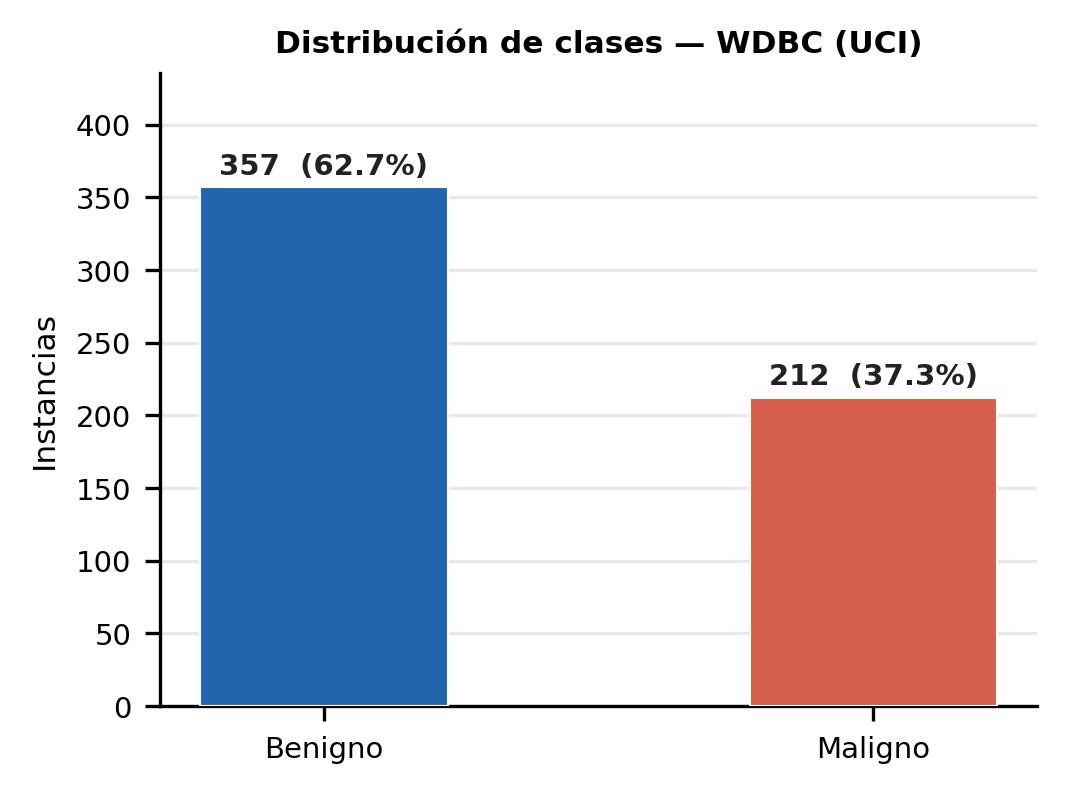
\includegraphics[width=0.85\textwidth]{../documento/images/fig_class_distribution.png}
\caption{\tiny Distribución de clases en WDBC}
\end{figure}
\end{column}
\end{columns}

\vspace{0.5em}
\begin{alertblock}{Trampa del accuracy}
Un clasificador que siempre prediga ``benigno'' obtendría 62.7\% de exactitud \textbf{sin detectar ningún tumor maligno}.
\end{alertblock}
\end{frame}

% ------------------------------------------------------------------------------
\section{Metodología}
% ------------------------------------------------------------------------------

\begin{frame}{Flujo metodológico}
\begin{center}
\begin{tabular}{cl}
\toprule
\textbf{Fase} & \textbf{Descripción} \\
\midrule
1. EDA & Análisis Exploratorio de Datos \\
2. Preprocesamiento & Detección de anómalos, normalización z-score \\
3. Selección de atributos & Intersección de 2 métodos \\
4. División de datos & 75\% entrenamiento / 25\% prueba \\
5. Modelado & 9 clasificadores ML \\
6. Evaluación & Recall Maligno como métrica principal \\
\bottomrule
\end{tabular}
\end{center}
\end{frame}

\begin{frame}{Análisis Exploratorio (EDA)}
\begin{columns}
\begin{column}{0.5\textwidth}
\begin{block}{Mapa de correlación}
Se identifican \textbf{bloques de alta correlación} entre las versiones \textit{mean}, \textit{error} y \textit{worst} de los mismos atributos.

\vspace{0.5em}
\textbf{Implicación:} redundancia que justifica selección de atributos.
\end{block}

\vspace{0.5em}
\begin{block}{Distribuciones por clase}
\begin{itemize}
  \item \texttt{mean area}, \texttt{mean concavity}: alta separación
  \item \texttt{mean texture}: considerable solapamiento
\end{itemize}
\end{block}
\end{column}

\begin{column}{0.5\textwidth}
\begin{figure}
\centering
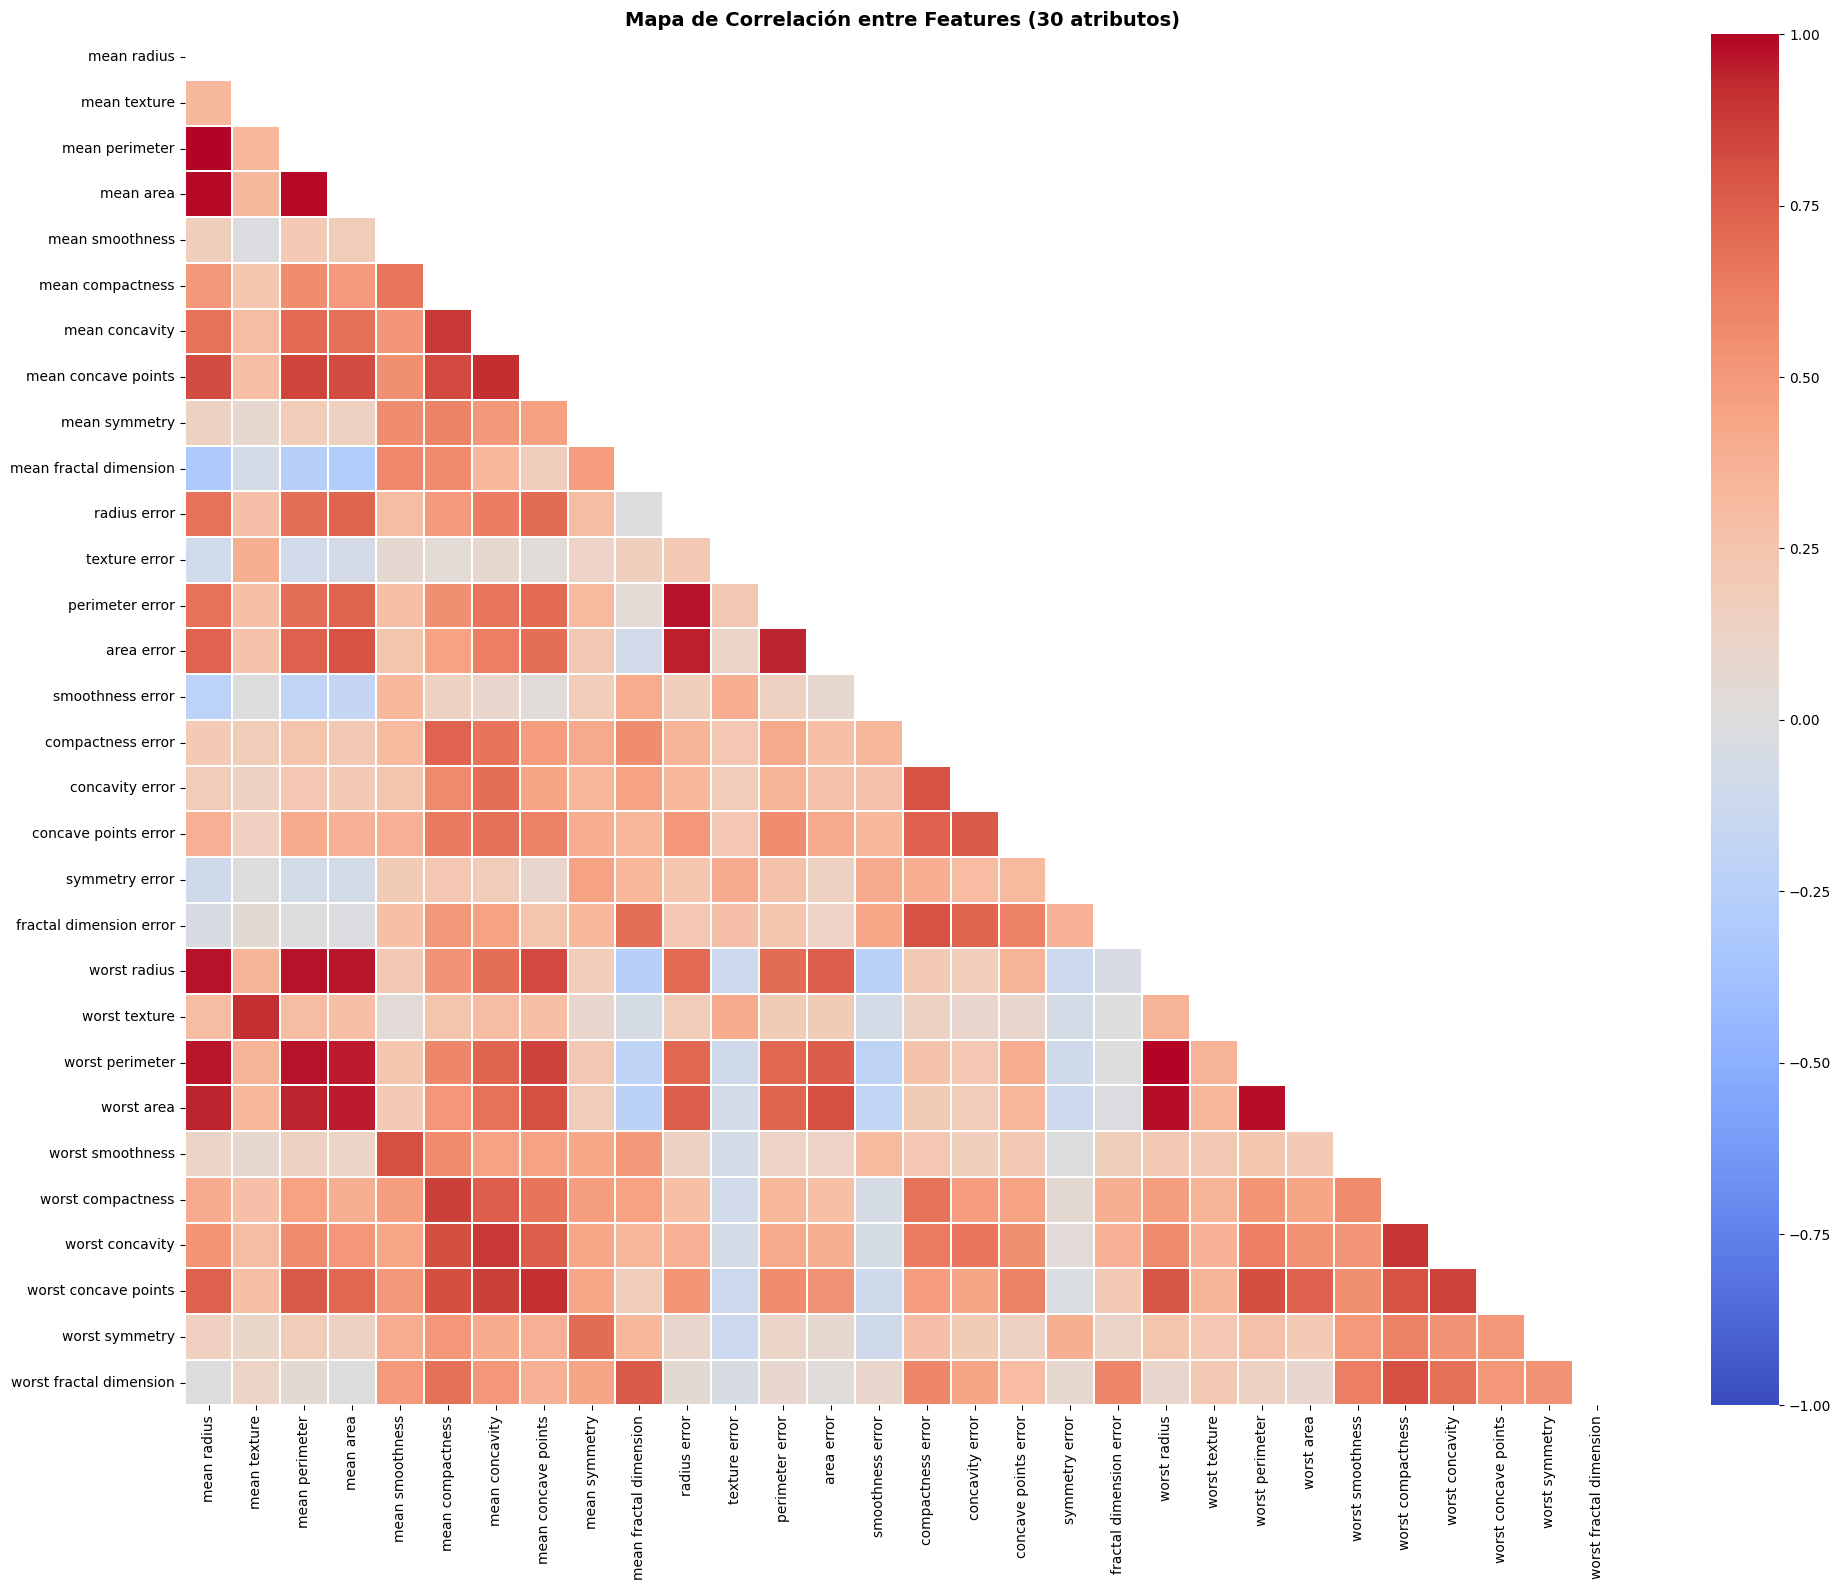
\includegraphics[width=0.85\textwidth]{../documento/images/fig_correlation_heatmap.png}
\caption{\tiny Mapa de correlación (30 características)}
\end{figure}
\end{column}
\end{columns}
\end{frame}

\begin{frame}{Distribuciones de características clave}
\begin{figure}
\centering
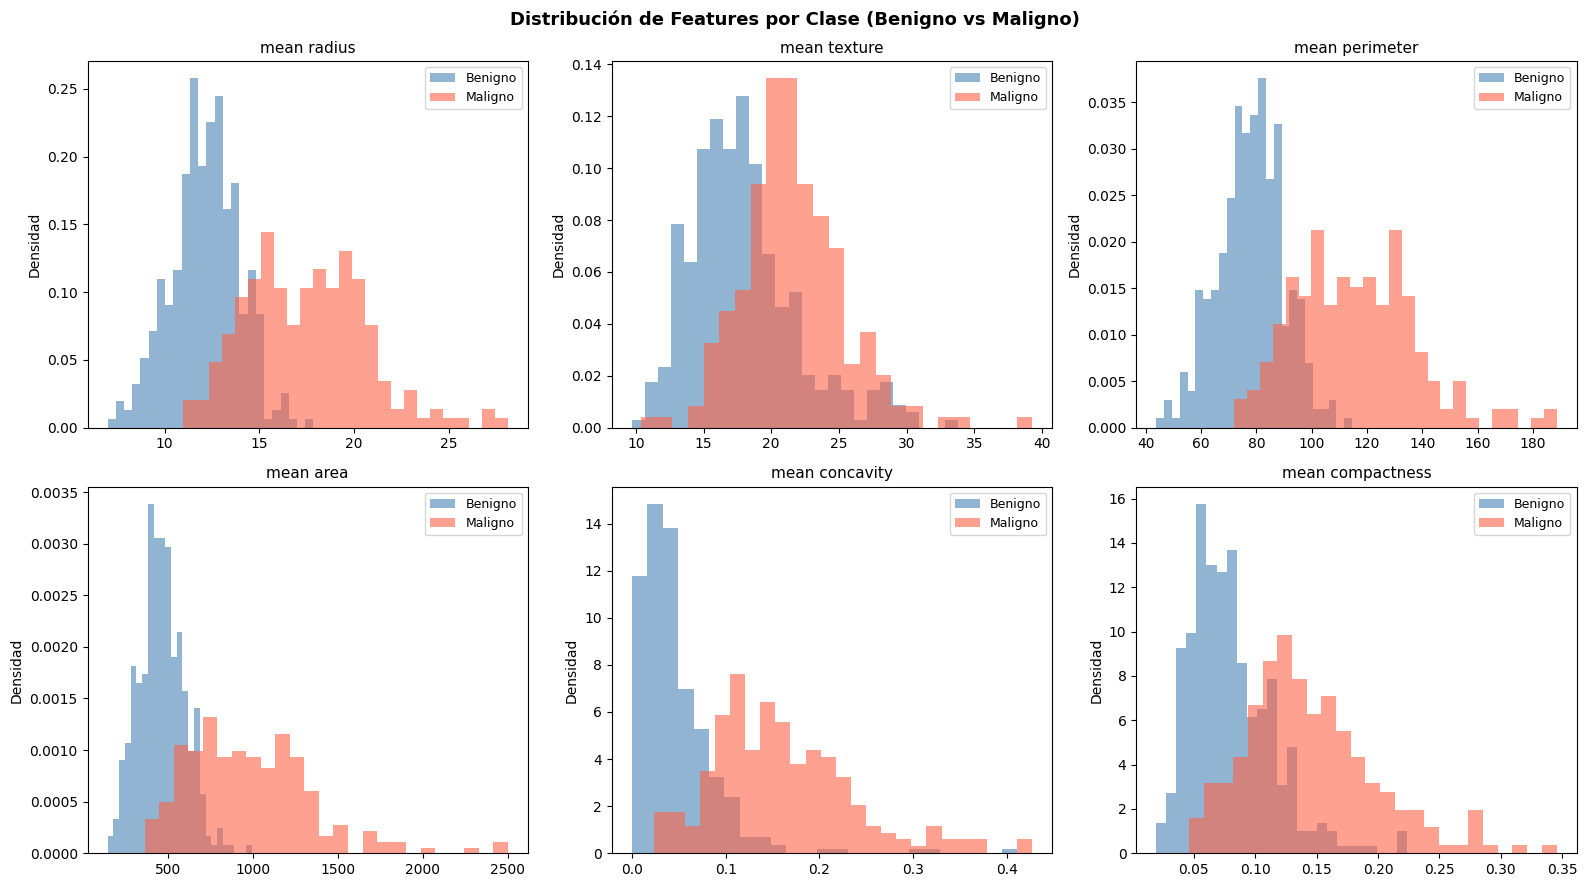
\includegraphics[width=0.7\textwidth]{../documento/images/fig_feature_distributions.png}
\caption{Distribución de características clave por clase. Menor solapamiento = mayor poder discriminativo.}
\end{figure}
\end{frame}

\begin{frame}{Preprocesamiento}
\begin{columns}
\begin{column}{0.5\textwidth}
\begin{block}{Detección de valores anómalos}
Regla de tres sigma: $\mu \pm 3\sigma$
\begin{itemize}
  \item 74 instancias detectadas (13\%)
  \item \textbf{Decisión: se conservan} -- son mediciones clínicas válidas
  \item Eliminarlos sesgaría el modelo contra tumores atípicos
\end{itemize}
\end{block}
\end{column}

\begin{column}{0.5\textwidth}
\begin{block}{Normalización z-score}
\begin{equation*}
z = \frac{x - \mu}{\sigma}
\end{equation*}
\begin{itemize}
  \item Escalador ajustado \textbf{únicamente} en entrenamiento
  \item Evita \textit{data leakage}
  \item Indispensable para SVM y KNN
\end{itemize}
\end{block}
\end{column}
\end{columns}
\end{frame}

% ------------------------------------------------------------------------------
\section{Selección de Atributos}
% ------------------------------------------------------------------------------

\begin{frame}{Intersección de dos métodos}
\begin{block}{Técnica 1: Correlación con la variable objetivo}
$|r| \geq 0.50$ $\rightarrow$ 16 características
\end{block}

\vspace{0.5em}
\begin{block}{Técnica 2: Separación de medias}
$TEST = \frac{|\bar{x}_B - \bar{x}_M|}{SE(A-B)} \geq 3.0$ $\rightarrow$ 16 características
\end{block}

\vspace{0.5em}
\begin{alertblock}{Resultado}
\textbf{Intersección: 15 características} (reducción del 50\%)

Un atributo es relevante \textit{solo} si pasa \textbf{ambos} filtros.
\end{alertblock}
\end{frame}

\begin{frame}{Visualización de los métodos}
\begin{columns}
\begin{column}{0.5\textwidth}
\begin{figure}
\centering
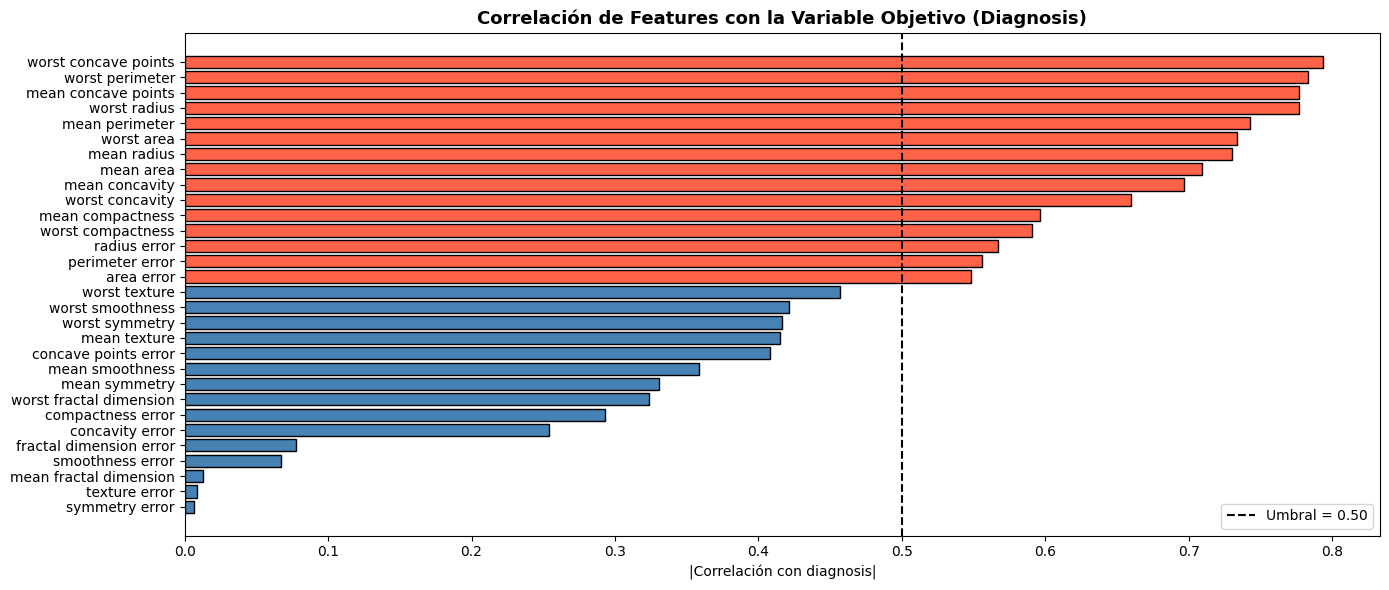
\includegraphics[width=0.9\textwidth]{../documento/images/fig_correlation_target.png}
\caption{\tiny Correlación con la variable objetivo}
\end{figure}
\end{column}

\begin{column}{0.5\textwidth}
\begin{figure}
\centering
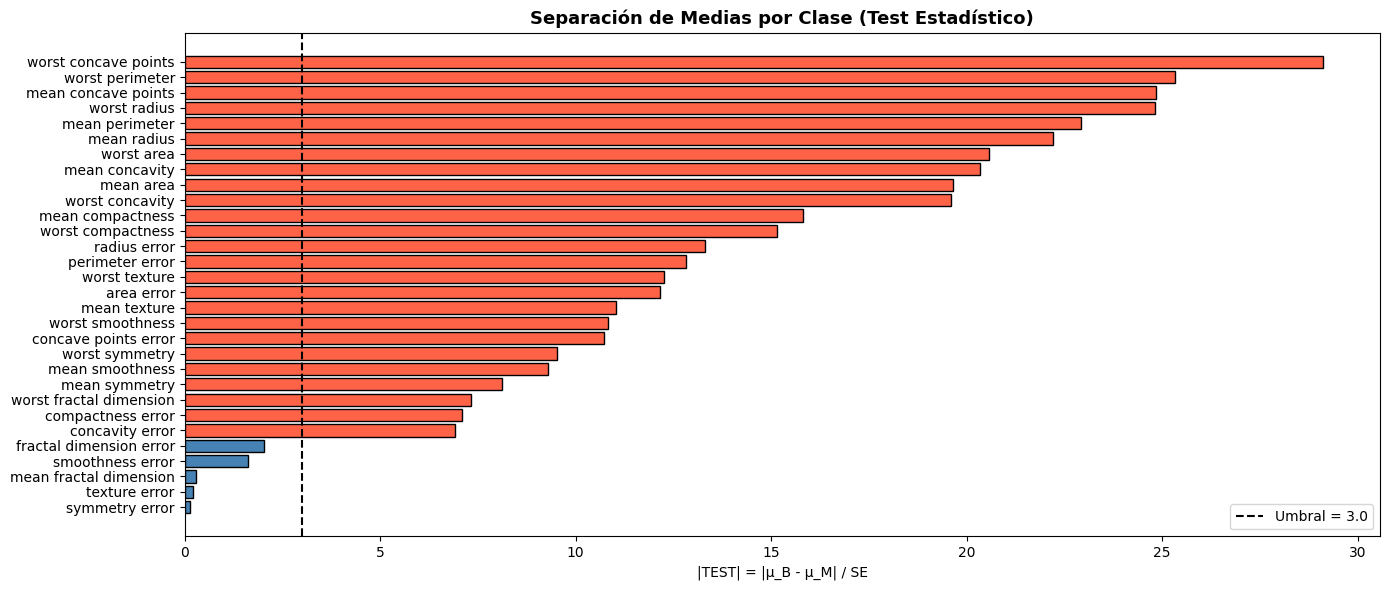
\includegraphics[width=0.9\textwidth]{../documento/images/fig_mean_variance_test.png}
\caption{\tiny Prueba de separación de medias}
\end{figure}
\end{column}
\end{columns}
\end{frame}

\begin{frame}{15 características seleccionadas}
\begin{center}
\small
\begin{tabular}{clcl}
\toprule
\# & Característica & \# & Característica \\
\midrule
1 & area error & 9 & radius error \\
2 & mean area & 10 & worst area \\
3 & mean compactness & 11 & worst compactness \\
4 & mean concave points & 12 & worst concave points \\
5 & mean concavity & 13 & worst concavity \\
6 & mean perimeter & 14 & worst perimeter \\
7 & mean radius & 15 & worst radius \\
8 & perimeter error & & \\
\bottomrule
\end{tabular}
\end{center}

\vspace{0.5em}
\textbf{Descartadas:} texture, smoothness, symmetry, fractal dimension (menor poder discriminativo, confirmado por el EDA).
\end{frame}

% ------------------------------------------------------------------------------
\section{Métrica Principal}
% ------------------------------------------------------------------------------

\begin{frame}{Recall de la clase Maligno}
\begin{columns}
\begin{column}{0.5\textwidth}
\begin{block}{Definición}
\begin{equation*}
\text{Recall Maligno} = \frac{TP}{TP + FN}
\end{equation*}
\textbf{Sensibilidad:} ¿qué fracción de tumores malignos detectamos?
\end{block}
\end{column}

\begin{column}{0.5\textwidth}
\begin{alertblock}{¿Por qué esta métrica?}
\begin{itemize}
  \item \textbf{FN}: tumor maligno como benigno $\rightarrow$ \textbf{no tratar}
  \item \textbf{FP}: tumor benigno como maligno $\rightarrow$ exámenes adicionales
  \item El riesgo del FN es \textbf{sustancialmente mayor}
  \item Todas las decisiones de hiperparámetros se optimizaron sobre este Recall
\end{itemize}
\end{alertblock}
\end{column}
\end{columns}
\end{frame}

% ------------------------------------------------------------------------------
\section{Modelos Implementados}
% ------------------------------------------------------------------------------

\begin{frame}{Los 9 clasificadores evaluados}
\begin{columns}
\begin{column}{0.5\textwidth}
\begin{itemize}
  \item SVM (kernel lineal)
  \item Regresión Logística
  \item Árbol de Decisión
  \item Random Forest (100 árboles)
  \item KNN
\end{itemize}
\end{column}

\begin{column}{0.5\textwidth}
\begin{itemize}
  \item Naive Bayes Gaussiano
  \item XGBoost
  \item AdaBoost
  \item ANN (3 capas densas)
\end{itemize}
\end{column}
\end{columns}

\vspace{1em}
\begin{block}{Condiciones experimentales idénticas}
\begin{itemize}
  \item Mismas 15 características seleccionadas
  \item Mismo conjunto de prueba (143 instancias)
  \item Implementación en scikit-learn y Keras/TensorFlow
\end{itemize}
\end{block}
\end{frame}

\begin{frame}{Regresión Logística -- \textbf{Mejor modelo}}
\begin{columns}
\begin{column}{0.5\textwidth}
\begin{exampleblock}{Resultados}
\begin{itemize}
  \item \textbf{Exactitud}: 97.90\%
  \item \textbf{Precisión Maligno}: 1.000 (cero falsos positivos)
  \item \textbf{Recall Maligno}: 0.9434 -- \textbf{mejor del experimento}
  \item Falsos negativos: solo 3 de 53
\end{itemize}
\end{exampleblock}

\vspace{0.5em}
CV Recall = $0.899 \pm 0.012$ (estable)

\vspace{0.5em}
\textbf{Coeficientes interpretables} que permiten auditar cada decisión clínica.
\end{column}

\begin{column}{0.5\textwidth}
\begin{figure}
\centering
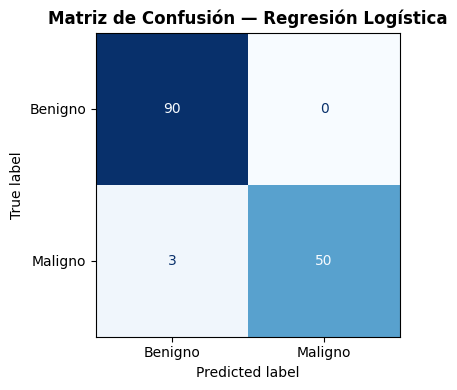
\includegraphics[width=0.85\textwidth]{../documento/images/regresion_logistica.png}
\caption{\tiny Matriz de confusión -- RL}
\end{figure}
\end{column}
\end{columns}
\end{frame}

\begin{frame}{XGBoost -- Segundo mejor}
\begin{columns}
\begin{column}{0.5\textwidth}
\begin{block}{Resultados}
\begin{itemize}
  \item Exactitud: 96.5\%
  \item Precisión Maligno: 0.980
  \item \textbf{Recall Maligno}: 0.925 -- \textbf{2° mejor}
  \item Falsos negativos: 4
\end{itemize}
\end{block}

\vspace{0.5em}
CV Recall = $0.893 \pm 0.046$ (mayor varianza)
\end{column}

\begin{column}{0.5\textwidth}
\begin{figure}
\centering
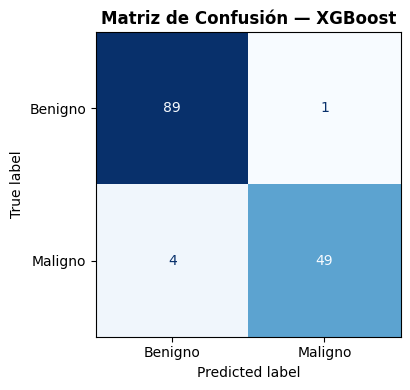
\includegraphics[width=0.8\textwidth]{../documento/images/fig_confusion_xgb.png}
\caption{\tiny Matriz de confusión -- XGBoost}
\end{figure}
\end{column}
\end{columns}
\end{frame}

\begin{frame}{SVM, Random Forest y ANN -- Tercer bloque}
\begin{columns}
\begin{column}{0.5\textwidth}
\begin{block}{Métricas idénticas}
\begin{itemize}
  \item Exactitud: 96.5\%
  \item Precisión Maligno: 1.000
  \item Recall Maligno: 0.906
  \item Cero falsos positivos
\end{itemize}
\end{block}

\vspace{0.5em}
\textbf{Diferencia clave: estabilidad}
\begin{itemize}
  \item Random Forest: CV $0.918 \pm 0.015$ -- \textbf{más estable}
  \item SVM: CV $0.893 \pm 0.046$ -- mayor varianza
\end{itemize}
\end{column}

\begin{column}{0.5\textwidth}
\begin{figure}
\centering
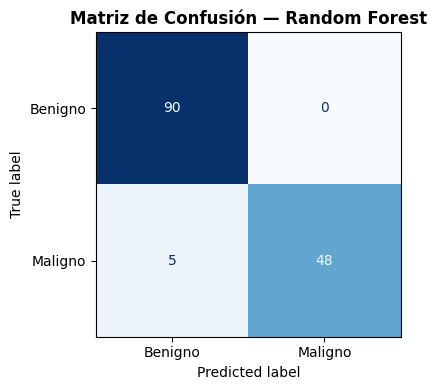
\includegraphics[width=0.8\textwidth]{../documento/images/fig_confusion_rf.png}
\caption{\tiny Matriz -- Random Forest}
\end{figure}
\end{column}
\end{columns}
\end{frame}

\begin{frame}{Random Forest -- Importancia de características}
\begin{columns}
\begin{column}{0.5\textwidth}
\begin{block}{Cuatro atributos dominantes}
\begin{itemize}
  \item \texttt{worst perimeter}
  \item \texttt{worst area}
  \item \texttt{worst concave points}
  \item \texttt{worst radius}
\end{itemize}
\end{block}

\vspace{0.5em}
\textbf{Concentran el 56.2\%} del poder predictivo total.

\vspace{0.5em}
La morfología más extrema de las células es el factor más discriminativo.
\end{column}

\begin{column}{0.5\textwidth}
\begin{figure}
\centering
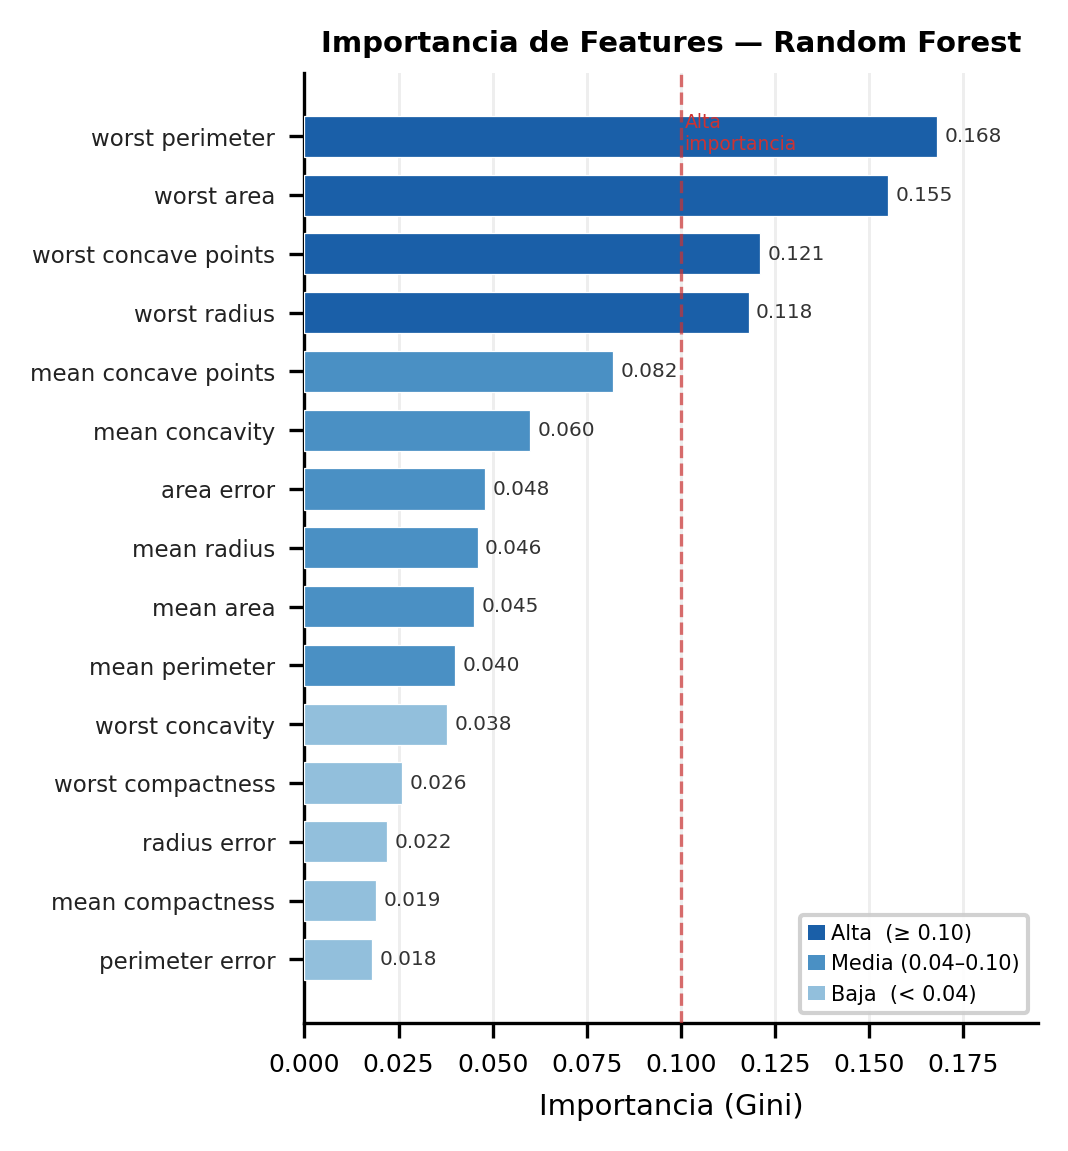
\includegraphics[width=0.65\textwidth]{../documento/images/fig_rf_importances.png}
\caption{\tiny Importancia Gini -- Random Forest}
\end{figure}
\end{column}
\end{columns}
\end{frame}

\begin{frame}{KNN y Naive Bayes}
\begin{columns}
\begin{column}{0.5\textwidth}
\begin{block}{KNN ($k$=1)}
\begin{itemize}
  \item Exactitud: 90.9\%
  \item Recall Maligno: 0.849
  \item FP: 5 (mayor cantidad del experimento)
  \item Muy sensible al ruido con $k=1$
\end{itemize}
\end{block}
\end{column}

\begin{column}{0.5\textwidth}
\begin{block}{Naive Bayes Gaussiano}
\begin{itemize}
  \item Exactitud: 93.7\%
  \item Recall Maligno: 0.849
  \item CV Recall: $0.880 \pm 0.013$ -- \textbf{más estable}
  \item Conservador: favorece especificidad sobre sensibilidad
\end{itemize}
\end{block}
\end{column}
\end{columns}
\end{frame}

\begin{frame}{AdaBoost y Árbol de Decisión}
\begin{columns}
\begin{column}{0.5\textwidth}
\begin{block}{AdaBoost}
\begin{itemize}
  \item Exactitud: 94.4\%
  \item Recall Maligno: 0.868
  \item 7 falsos negativos
  \item CV Recall: $0.893 \pm 0.031$
\end{itemize}
\end{block}
\end{column}

\begin{column}{0.5\textwidth}
\begin{alertblock}{Árbol de Decisión}
\begin{itemize}
  \item Exactitud: 92.3\%
  \item Recall Maligno: \textbf{0.830 -- más bajo}
  \item \textbf{Ventaja:} máxima interpretabilidad
  \item Reglas SI--ENTONCES auditables por médicos
\end{itemize}
\end{alertblock}
\end{column}
\end{columns}
\end{frame}

\begin{frame}{Red Neuronal Artificial (ANN)}
\begin{columns}
\begin{column}{0.5\textwidth}
\begin{block}{Arquitectura}
\begin{itemize}
  \item 3 capas densas (16-16-1)
  \item 545 parámetros entrenables
  \item Dropout 20\% + Early Stopping
\end{itemize}
\end{block}

\vspace{0.5em}
\begin{block}{Resultados}
\begin{itemize}
  \item Exactitud: 96.5\%
  \item Precisión Maligno: 1.000
  \item Recall Maligno: 0.906
\end{itemize}
\end{block}

\vspace{0.5em}
\textbf{Sorpresa:} no supera a modelos lineales. El problema es linealmente separable.
\end{column}

\begin{column}{0.35\textwidth}
\begin{figure}
\centering
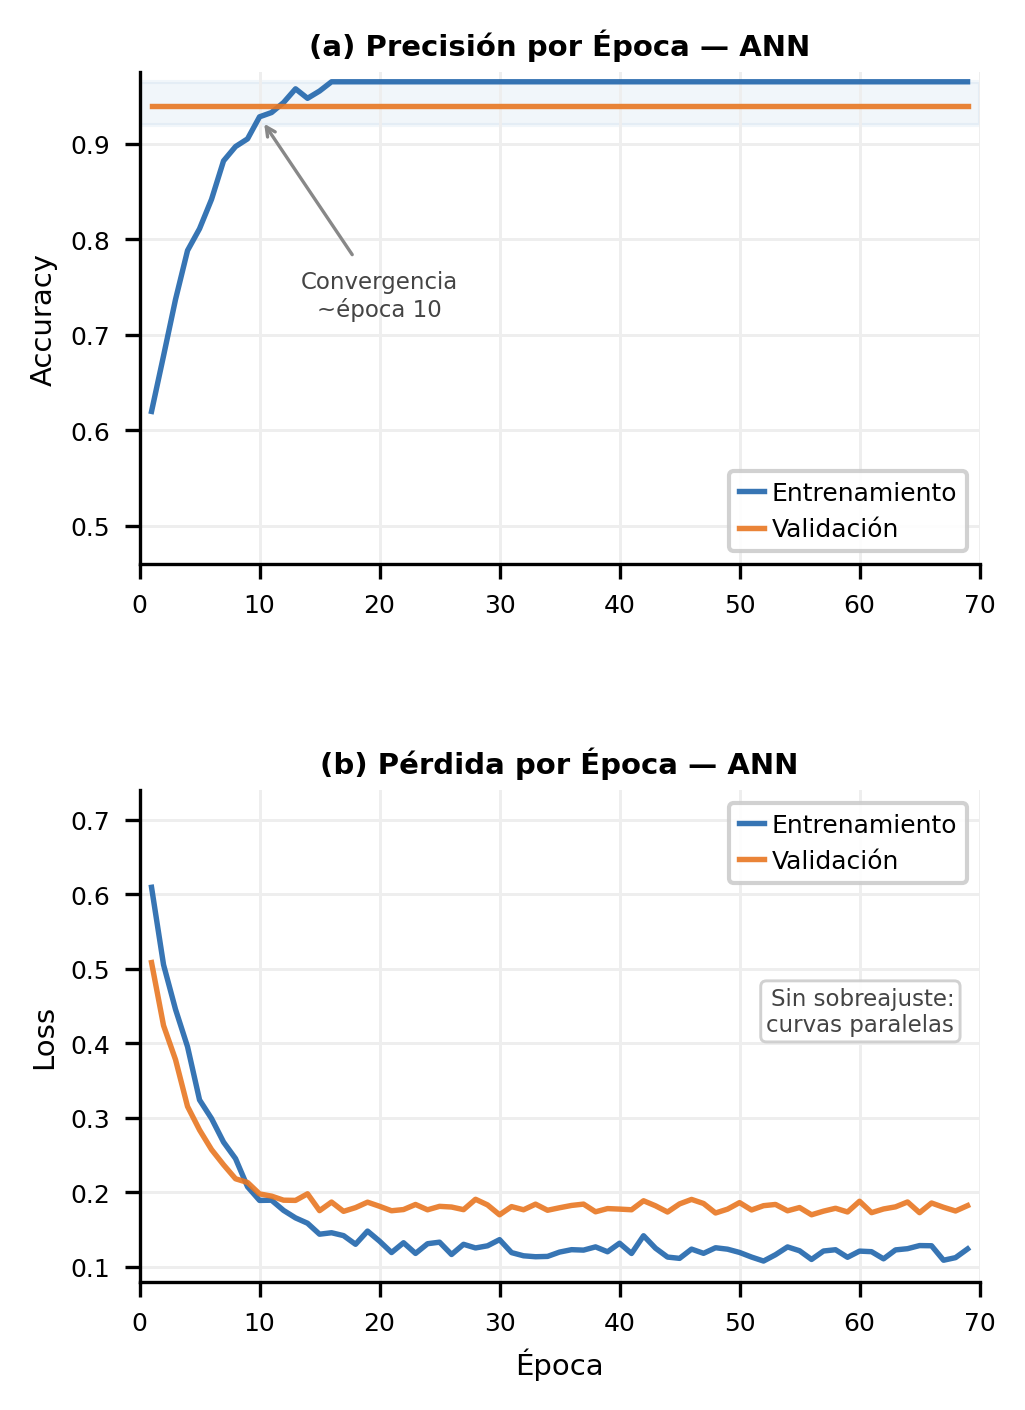
\includegraphics[width=0.8\textwidth]{../documento/images/fig_ann_training.png}
\caption{\tiny Curvas de entrenamiento ANN}
\end{figure}
\end{column}
\end{columns}
\end{frame}

% ------------------------------------------------------------------------------
\section{Resultados Comparativos}
% ------------------------------------------------------------------------------

\begin{frame}{Ranking por Recall Maligno}
\begin{columns}
\begin{column}{0.45\textwidth}
\begin{block}{Posiciones}
\begin{enumerate}
  \item \textbf{Reg. Logística: 0.9434}
  \item XGBoost: 0.9245
  \item SVM, ANN, RF: 0.9057
  \item AdaBoost: 0.8679
  \item Naive Bayes, KNN: 0.8491
  \item Árbol Decisión: 0.8302
\end{enumerate}
\end{block}
\end{column}

\begin{column}{0.55\textwidth}
\begin{figure}
\centering
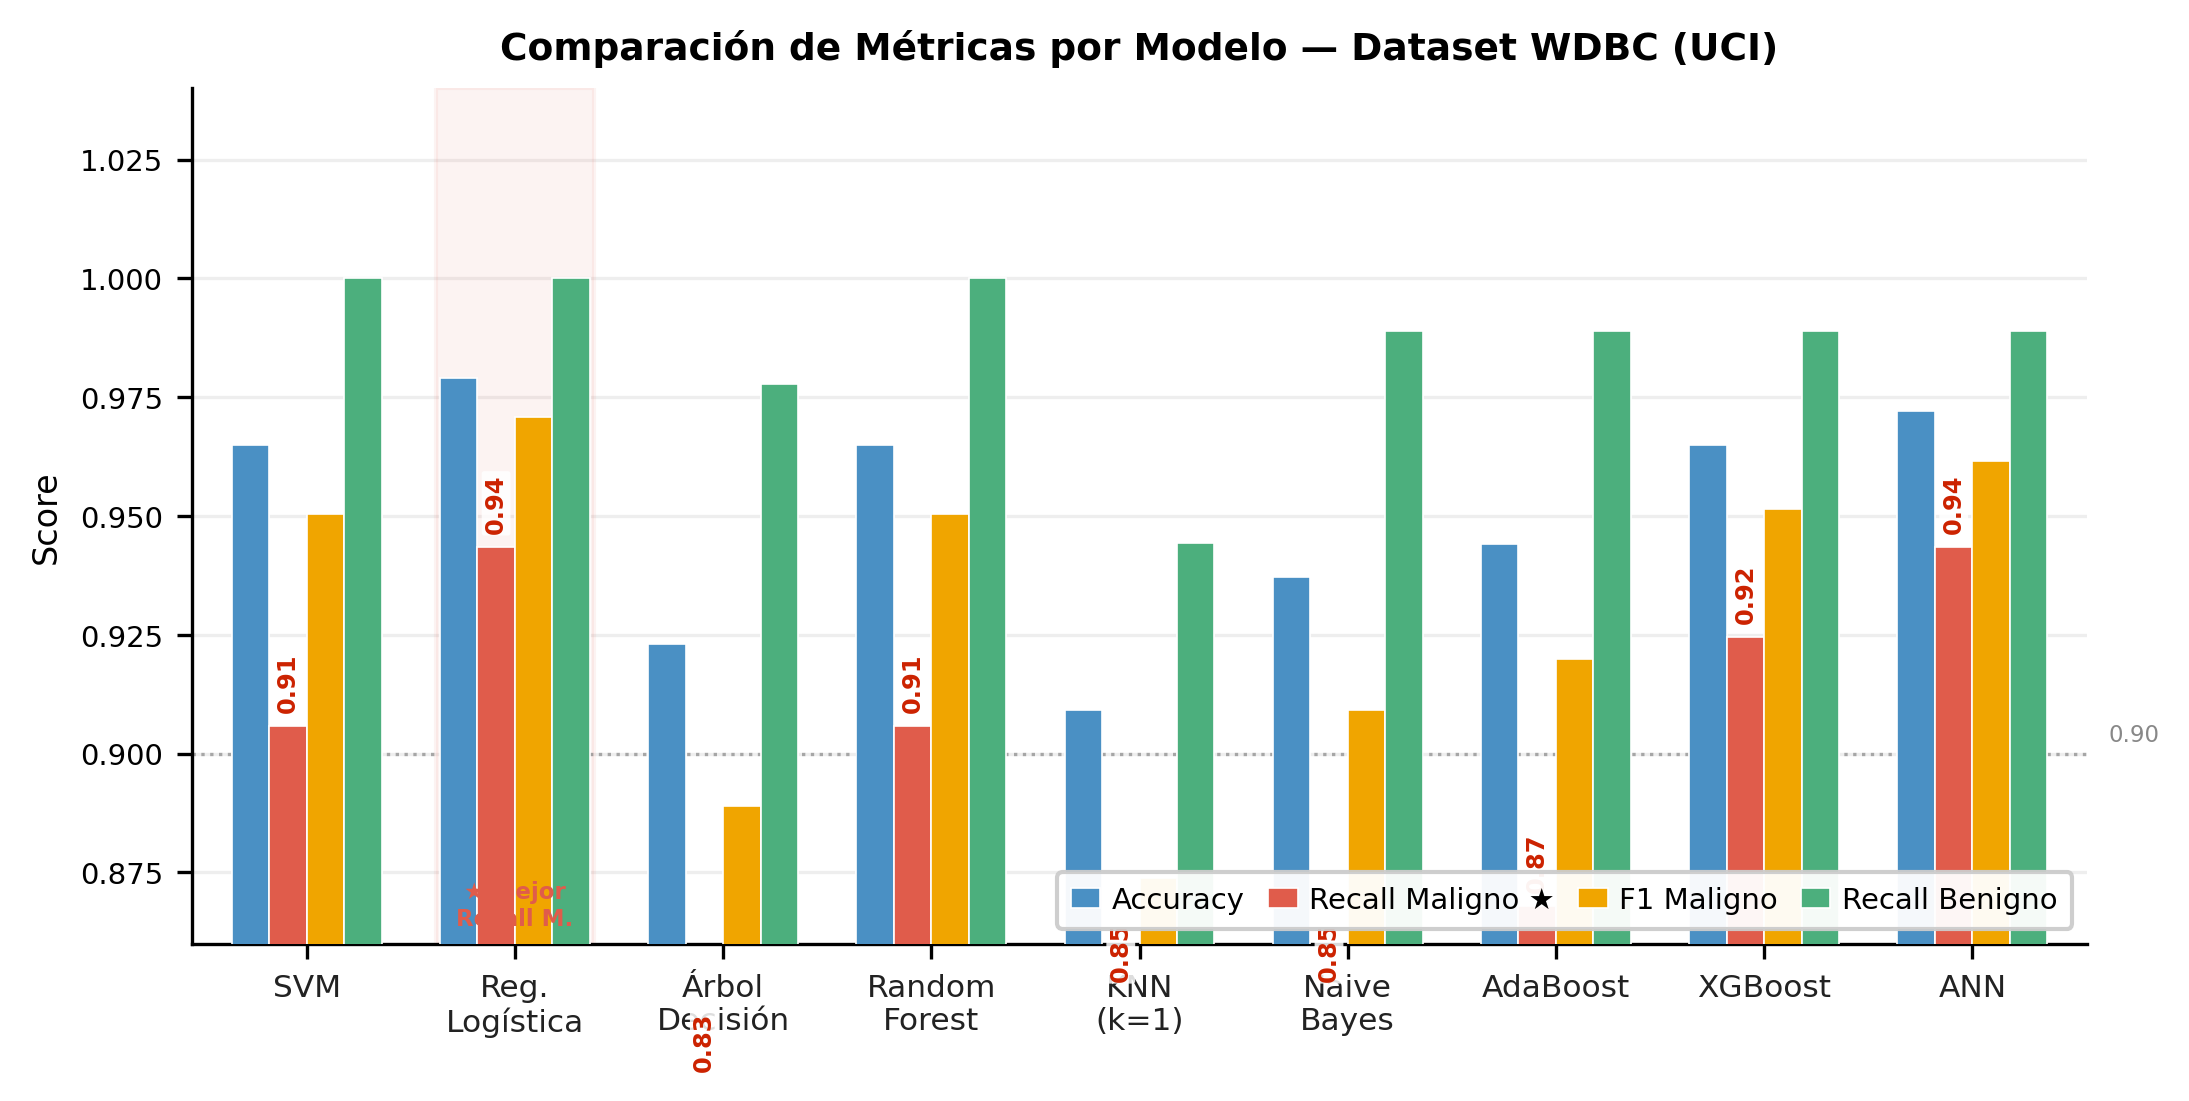
\includegraphics[width=0.85\textwidth]{../documento/images/fig_metrics_comparison.png}
\caption{\tiny Comparación visual de métricas}
\end{figure}
\end{column}
\end{columns}
\end{frame}

\begin{frame}{Curvas ROC}
\begin{figure}
\centering
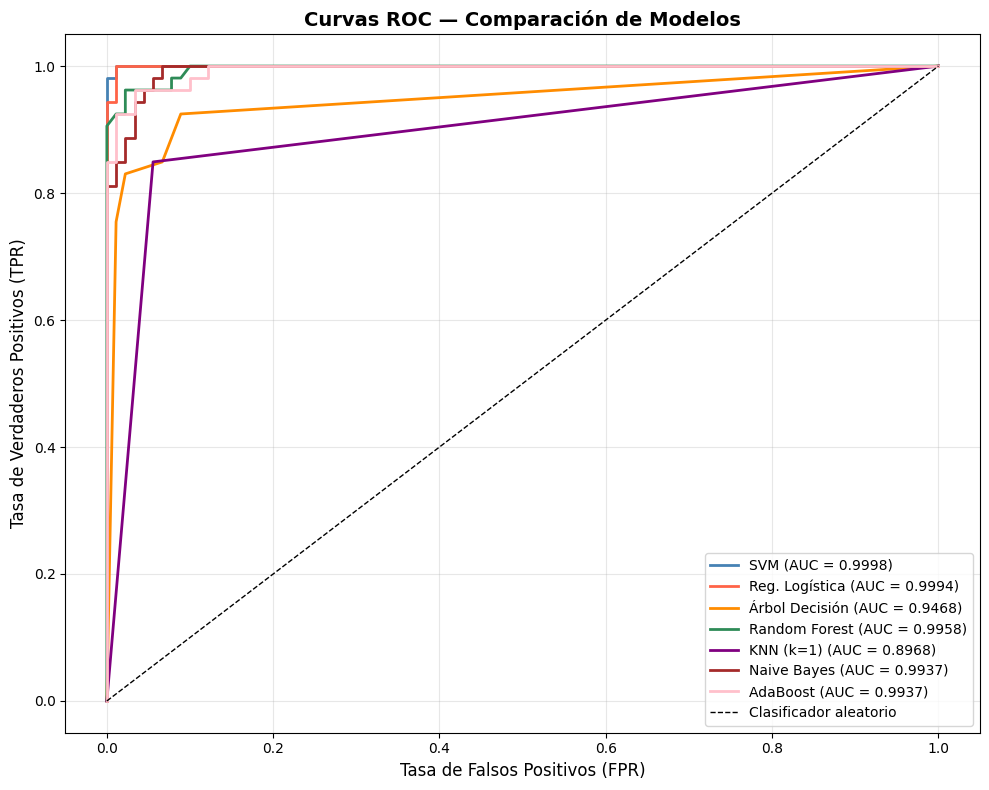
\includegraphics[width=0.35\textwidth]{../documento/images/fig_roc_curves.png}
\caption{Curvas ROC para 7 modelos evaluados}
\end{figure}

\vspace{0.3em}
\begin{center}
\small
AUC = probabilidad de que el modelo asigne mayor score a un maligno que a un benigno.
\end{center}
\end{frame}

\begin{frame}{Tabla comparativa completa}
\begin{center}
\scriptsize
\begin{tabular}{lcccc}
\toprule
\textbf{Modelo} & \textbf{Exactitud} & \textbf{Prec. M.} & \textbf{Recall M.} & \textbf{F1 M.} \\
\midrule
Reg. Logística & \cellcolor{verdemejor}0.979 & \cellcolor{verdemejor}1.000 & \cellcolor{verdemejor}0.943 & \cellcolor{verdemejor}0.971 \\
XGBoost & 0.965 & 0.980 & 0.925 & 0.952 \\
SVM & 0.965 & \cellcolor{verdemejor}1.000 & 0.906 & 0.951 \\
ANN & 0.965 & \cellcolor{verdemejor}1.000 & 0.906 & 0.951 \\
Random Forest & 0.965 & \cellcolor{verdemejor}1.000 & 0.906 & 0.951 \\
AdaBoost & 0.944 & 0.979 & 0.868 & 0.920 \\
Naive Bayes & 0.937 & 0.978 & 0.849 & 0.909 \\
KNN & \cellcolor{rojomenor}0.909 & \cellcolor{rojomenor}0.900 & 0.849 & \cellcolor{rojomenor}0.874 \\
Árbol Dec. & 0.923 & 0.957 & \cellcolor{rojomenor}0.830 & 0.889 \\
\bottomrule
\end{tabular}
\end{center}

\vspace{0.5em}
\begin{center}
\small Verde = mejor valor \hspace{1em} Rosa = peor valor por columna
\end{center}
\end{frame}

% ------------------------------------------------------------------------------
\section{Estabilidad y Generalización}
% ------------------------------------------------------------------------------

\begin{frame}{Validación cruzada 5-fold}
\begin{center}
\scriptsize
\begin{tabular}{lccc}
\toprule
\textbf{Modelo} & \textbf{Recall (prueba)} & \textbf{CV media} & \textbf{CV $\pm$ std} \\
\midrule
Reg. Logística & \cellcolor{verdemejor}0.943 & 0.931 & 0.025 \\
Random Forest & 0.906 & \cellcolor{verdemejor}0.918 & \cellcolor{verdemejor}0.015 \\
XGBoost & 0.925 & 0.893 & \cellcolor{rojomenor}0.046 \\
SVM & 0.906 & 0.893 & \cellcolor{rojomenor}0.046 \\
AdaBoost & 0.868 & 0.893 & 0.031 \\
Naive Bayes & 0.849 & 0.880 & \cellcolor{verdemejor}0.013 \\
KNN & 0.849 & 0.899 & 0.025 \\
Árbol Dec. & \cellcolor{rojomenor}0.830 & 0.855 & 0.039 \\
\bottomrule
\end{tabular}
\end{center}

\vspace{0.5em}
\begin{alertblock}{Insight clave}
SVM y Random Forest tienen \textbf{mismas métricas puntuales}, pero RF es 3 veces más estable en CV. La evaluación sobre un solo split habría ocultado esta diferencia.
\end{alertblock}
\end{frame}

\begin{frame}{Tres patrones de estabilidad}
\begin{block}{1. Alta sensibilidad, alta estabilidad}
\textbf{Regresión Logística} -- mejor Recall (0.943) con desviación moderada ($\pm$0.025). El problema es linealmente separable.
\end{block}

\vspace{0.5em}
\begin{block}{2. Alta sensibilidad, alta varianza}
\textbf{XGBoost} -- segundo mejor Recall (0.925) pero mayor desviación ($\pm$0.046). Riesgo en datasets pequeños.
\end{block}

\vspace{0.5em}
\begin{block}{3. Menor sensibilidad, mayor estabilidad}
\textbf{Naive Bayes} ($\pm$0.013) y \textbf{Random Forest} ($\pm$0.015). Predicciones altamente consistentes entre particiones.
\end{block}
\end{frame}

% ------------------------------------------------------------------------------
\section{Discusión y Conclusiones}
% ------------------------------------------------------------------------------

\begin{frame}{Conclusiones principales}
\begin{columns}
\begin{column}{0.5\textwidth}
\begin{block}{Sobre el flujo}
\begin{itemize}
  \item \textbf{EDA}: identificó redundancia entre versiones mean/error/worst
  \item \textbf{Normalización z-score}: indispensable para SVM y KNN
  \item \textbf{Selección}: reducción 50\% (30$\rightarrow$15) sin pérdida de rendimiento
  \item \textbf{Recall Maligno}: la métrica correcta para el contexto clínico
\end{itemize}
\end{block}
\end{column}

\begin{column}{0.5\textwidth}
\begin{exampleblock}{Sobre los modelos}
\begin{itemize}
  \item \textbf{Regresión Logística}: mejor modelo global (Recall 0.943, precisión perfecta)
  \item El problema es \textbf{linealmente separable} con las 15 características
  \item Modelos complejos (ANN, RF) \textbf{no superaron} a modelos lineales
  \item La \textbf{validación cruzada} distingue modelos con igual rendimiento puntual
\end{itemize}
\end{exampleblock}
\end{column}
\end{columns}
\end{frame}

\begin{frame}{Recomendaciones según el contexto}
\begin{columns}
\begin{column}{0.5\textwidth}
\begin{exampleblock}{Screening masivo}
\textbf{Regresión Logística} -- mayor Recall, coeficientes interpretables, cero falsos positivos.
\end{exampleblock}

\vspace{0.5em}
\begin{block}{Segunda opinión clínica}
\textbf{Random Forest} -- mejor estabilidad en CV ($\pm$0.015) con rendimiento competitivo.
\end{block}
\end{column}

\begin{column}{0.5\textwidth}
\begin{block}{Comunicación de riesgo}
\textbf{Naive Bayes} -- probabilidades posteriores explícitas $P(\text{Maligno}|\mathbf{x})$, mayor consistencia.
\end{block}

\vspace{0.5em}
\begin{alertblock}{Validación médica}
\textbf{Árbol de Decisión} -- reglas SI--ENTONCES auditables, a costa del menor Recall.
\end{alertblock}
\end{column}
\end{columns}
\end{frame}

\begin{frame}{Aprendizajes clave}
\begin{enumerate}
  \item La \textbf{exactitud es insuficiente} en problemas médicos con desbalance de clases.
  
  \item KNN: 90.9\% accuracy pero solo 84.91\% Recall Maligno -- \textbf{8 tumores malignos sin detectar}.
  
  \item La analítica de datos es un \textbf{proceso integrado}: preprocesamiento es tan determinante como el algoritmo.
  
  \item La \textbf{validación cruzada} permite distinguir modelos con igual rendimiento puntual pero diferente estabilidad.
  
  \item Que un modelo lineal supere a una red neuronal de 545 parámetros confirma que \textbf{la complejidad no garantiza mejor rendimiento}.
\end{enumerate}
\end{frame}

\begin{frame}{Limitaciones y trabajo futuro}
\begin{itemize}
  \item Dataset de un único centro médico -- limita generalización a otras poblaciones.
  \item Tamaño reducido (569 instancias) -- insuficiente para arquitecturas de deep learning más complejas.
  \item No incorpora factores de riesgo clínicos (edad, historial familiar, marcadores genéticos).
  \item Validación interna (train/test) -- se requiere validación externa sobre dataset independiente.
  \item ANN no incluida en validación cruzada por costo computacional.
\end{itemize}
\end{frame}

\begin{frame}{Resumen ejecutivo}
\begin{center}
\Large
\textbf{Regresión Logística} obtuvo el mejor Recall Maligno (94.34\%)\\
con precisión perfecta (1.000) y cero falsos positivos.
\end{center}

\vspace{1em}
\begin{center}
\large
El flujo integrado de analítica de datos demuestra que\\
\textbf{preprocesamiento + métricas correctas + validación robusta}\\
son tan importantes como el algoritmo de clasificación.
\end{center}
\end{frame}

\backmatter
\end{document}
